\documentclass[a4paper,11pt]{article}

\usepackage[utf8]{inputenc}

\usepackage{graphicx}
\usepackage{caption}
\usepackage{subcaption}

\usepackage{pgfplots}
\pgfplotsset{compat=1.18} 

\usepackage{comment}

\usepackage{gensymb}

\usepackage{url}

\usepackage{floatrow}
\newfloatcommand{capbtabbox}{table}[][\FBwidth]

\usepackage{amsmath}

\begin{document}

\title{
  \textbf{A Physical Model} \\
  construction of a simple model for atmospheric carbon
}
\author{Johan Montelius}
\date{\today}

\maketitle

\section*{Introduction}

The concentration of carbon dioxide has increased during the
last century and we have very good data that shows us the
concentration on a monthly basis during the last sixty years. The
reason is, given the current narrative, that this is all due to our
burning of fossil fuel.

If we look at the last sixty years the yearly atmospheric increase is
in average half our our yearly emissions. If we look at the
correlation shown in Fig. \ref{fig:correlation}, the general trend is
clearly seen but also how much the increase can vary. A year with
emissions equivalent to three ppm could result in anything from a half
to three and a half ppm of increase. The statistical average is not a
good predictor for a particular year.

\begin{figure}[ht!]
  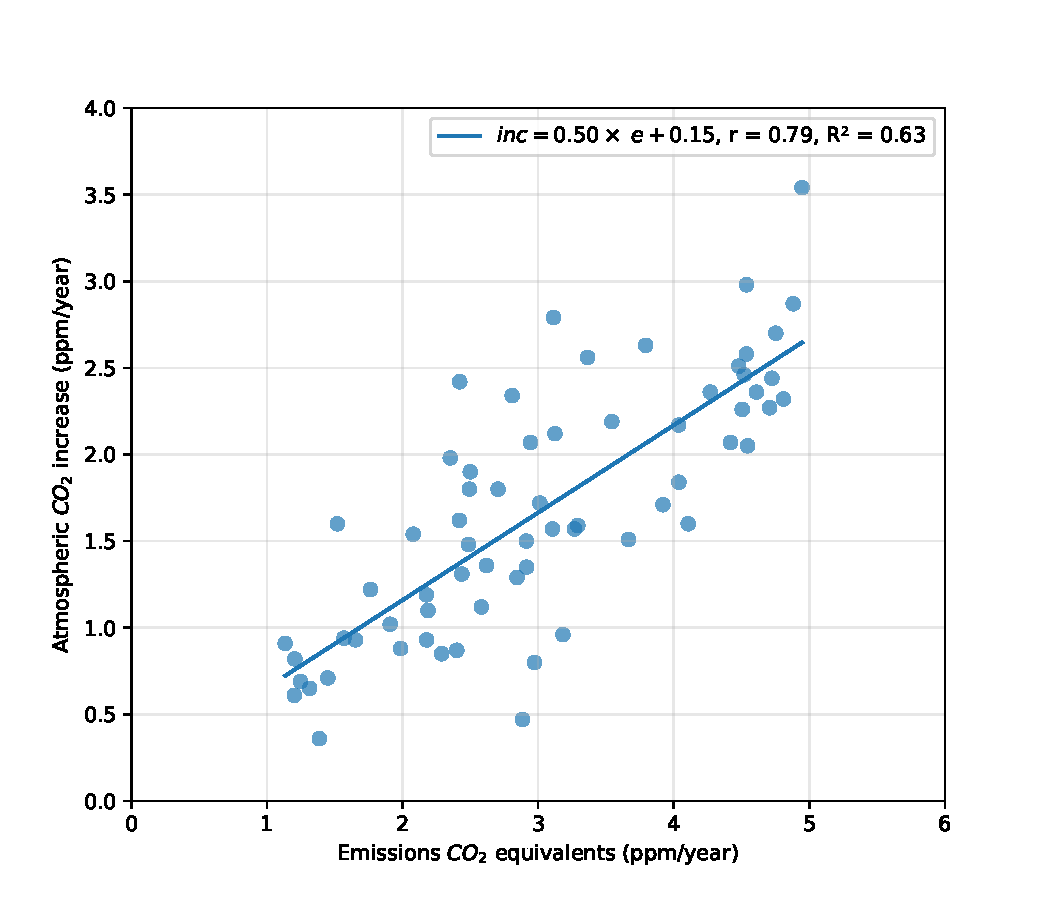
\includegraphics[scale=0.6]{../carbon/img/emissions-ppm.pdf}
  \caption{Correlation: emissions and atmospheric increase.}
  \label{fig:correlation}
\end{figure}

To better understand what is happening, and make predictions about the
future, we need a physical model that describe the processes
involved. The model will of course be a simplification of the real
world and that is expected. In fact the goal is to make it as simple
as possible while still capturing the changes that we are interested
in.


\section*{The atmosphere}

We start by examining the measurements of carbon dioxide
concentrations in the atmosphere from the Mauna Loa observatory on the
island of Hawaii \cite{noaa:co2}. The data that we will use is the
mean monthly measurements from $1958$ to $2026$ (full years from
$1959$ to $2025$). If we plot these data we will see the classical
{\em Keeling curve} as shown Fig. \ref{fig:keeling}.

\begin{figure}[t]
  \centering
  \hspace*{-4cm}
  \begin{subfigure}{.5\paperwidth}
    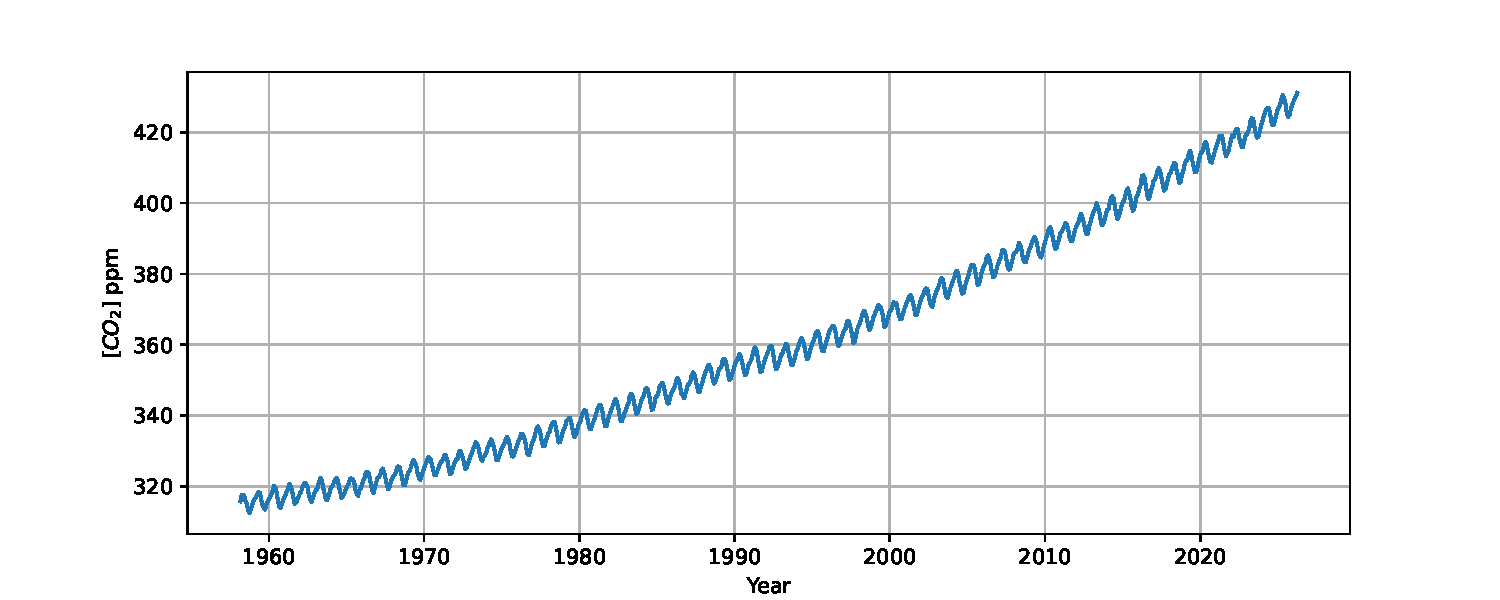
\includegraphics[scale=0.4]{../img/keeling.pdf}
    \caption{The Keeling curve}
    \label{fig:keeling}
  \end{subfigure}%
  \begin{subfigure}{.5\paperwidth}
    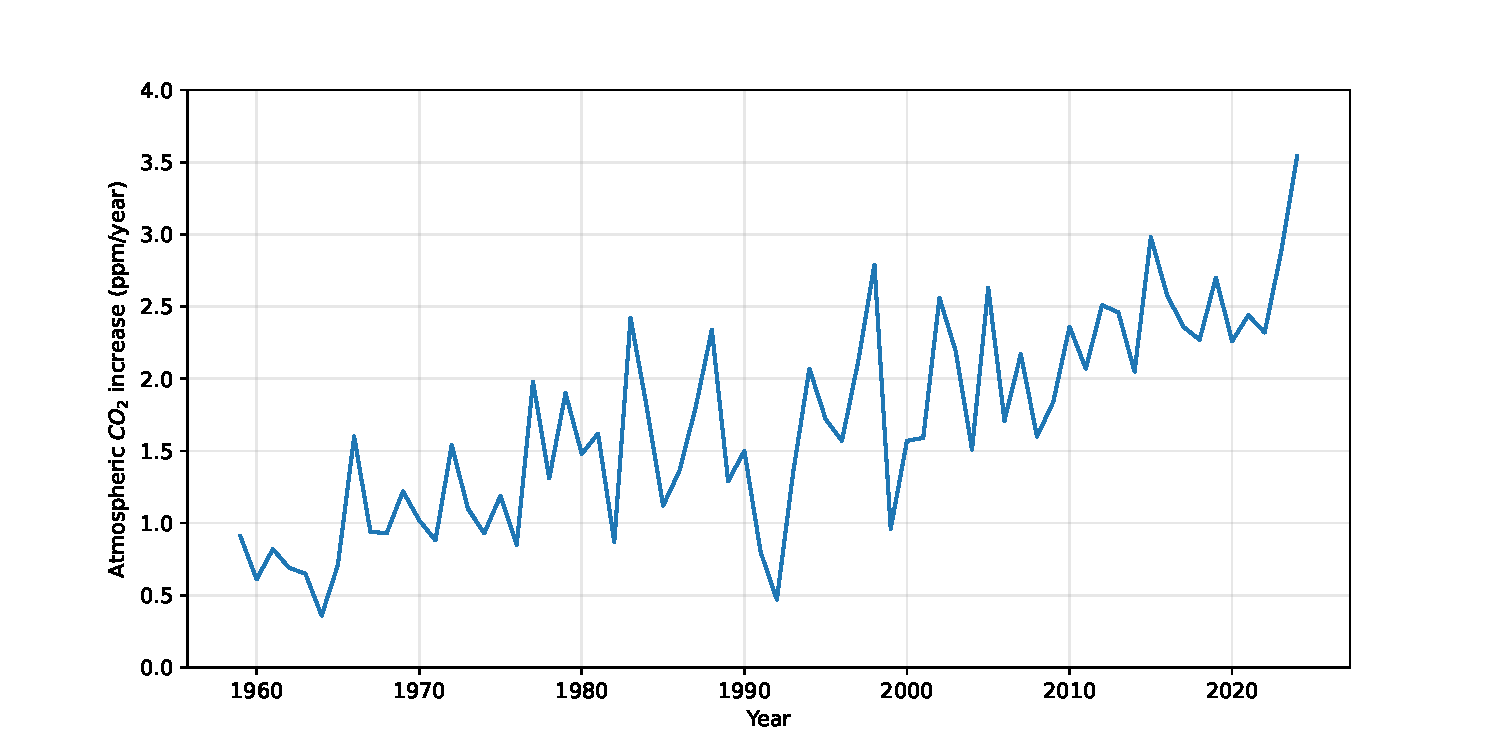
\includegraphics[scale=0.4]{../img/increase.pdf}
    \caption{December-December growth.}
    \label{fig:increase}
  \end{subfigure}
  \caption{Carbon dioxide concentration in the atmosphere..}
\end{figure}

The yearly increase is not as uniform as one would suspect but, as can
be seen in Fig. \ref{fig:increase} varies between less than half a ppm
to three and a half ppm.

The atmosphere is of course in constant contact to land and oceans,
large carbon reservoirs, earth so carbon dioxide in the atmosphere is
part of the large {\em carbon cycle}. Understanding this cycle is of
course key in being able to predict how the atmosphere will be
effected by human emissions. The model we should build does not have
to make prediction of all reservoirs as long as it helps us making
predictions about the atmosphere. 

\subsection*{the simplest model}

The simplest model we can make is a two-box model where one box
represents the atmosphere and the other the combination of land,
vegetation, volcanoes and oceans. Since the earth surface to 70\%
consist of water, for simplicity we can call this box {\em the
  oceans}. We assume that both boxes are well mixed and that the
transport from one box to the other is given by the concentration of
carbon in the originating box. We are here talking about to separate
flows not the net flow.

We know that this model is an oversimplification of the world since
vegetation behaves very different from oceans and that the oceans
themselves are stratified into layers where the surface layer is not
well mixed with the deep oceans. We also know that areas around the
equator behave very different from the polar regions so we should not
be surprised if our model does not work.

More advanced models will divide the biosphere from the oceans and
then divide the oceans into surface layer and deep oceans. The surface
layer is then divided in into high- and low-latitude boxes and the
interchange between these ocean layers is described both by {\em
  diffusion} i.e. the box is not well mixed, and {\em advection}
i.e. ocean currents. These model however, aspire to also describe what
is happening in the biosphere and oceans, not only what is happening in
the atmosphere. If we are only interested in the atmosphere, a simple
two-box model might be sufficient.

\subsection*{the unknowns}

If we want to know how the atmosphere reacts when we add carbon
dioxide through emissions we need to know the following: the amount of
carbon in the atmosphere and the oceans, and the flow in both
directions. If we, for sake of the argument, assume that the amount of
carbon in the oceans is forty times the amount in the atmosphere, then
we can predict what will happen with 10 gigaton of carbon that we emit
during a year.Eventually the 10 gigaton will, as all carbon, be
distributed in the ratio 1:50. How long time this will take depends on
the flow between the reservoirs. If 10\% of the carbon in the
atmosphere enters the oceans each year and $0.2\%$ of the carbon in
the oceans enters the atmosphere we will see a decrease of the extra
carbon in the atmosphere and after some decades we will find some
$0.2$ GtC still in the atmosphere and the remaining $9.8$ in the
oceans.

Of the parameters the only one that we can no with some certainty is
the amount of carbon in the atmosphere. We know this since we can
measure the mole concentration in the atmosphere and make a fair
judgment on the size of the atmosphere. Given a concentration of $428$
ppm this would mean approximately $428 * 2.13 \approx 912$ GtC. The
transport to and from the atmosphere is much harder to estimate but
most sources would agree on a number in the hundreds if both ocean and
vegetation is included. The size of the oceans is normally given as
around $40.000$ GtC so our example was probably not that far of
reality.

The problem is of course to more accurately determine the size of the
oceans, or rather the size of the other reservoir since it is a
collection of oceans and vegetation etc. We also need to determine the
size of the flows, up and down. If we can do this we can give a
prediction of what will happen with a 10 GtC of emissions.

\section*{Setting the stage}

To determine the unknowns we could set up an experiment. We could emit
a gigaton of colored carbon dioxide in the atmosphere and see what
is happening. The rate of decline of colored carbon in the atmosphere
would give us an estimate on the two flows, up and down, and the point
were it levels off would tell us how large the oceans are. This is
probably nothing that we would get permissions for and it would
probably take half a century before we would be able to draw any
conclusions.

\subsection*{the bomb curve}

Fortunately, this experiment has already been performed and it was
performed in the beginning of the sixties. In the late fifties to 1963
a total of over 500 atomic bombs were tested in the atmosphere. In
1963 a treaty was signed that banned all nuclear tests in the
atmosphere. A nuclear explosion will emit high energy neutrons that
when the hit a nitrogen atom will convert this atom to a carbon-14
(14C) isotope. Carbon consists almost solely of 12C and only one isotope
in a trillion is a 14C isotope. The atmosphere thus only contains less
than a ton of 14C but in the late fifties until 1965 this almost
doubled. We did thus actually "color" the carbon in the atmosphere and
now have the result.

\begin{figure}[ht!]
  \centering
  \hspace*{-4cm}
  \begin{subfigure}{.5\paperwidth}
    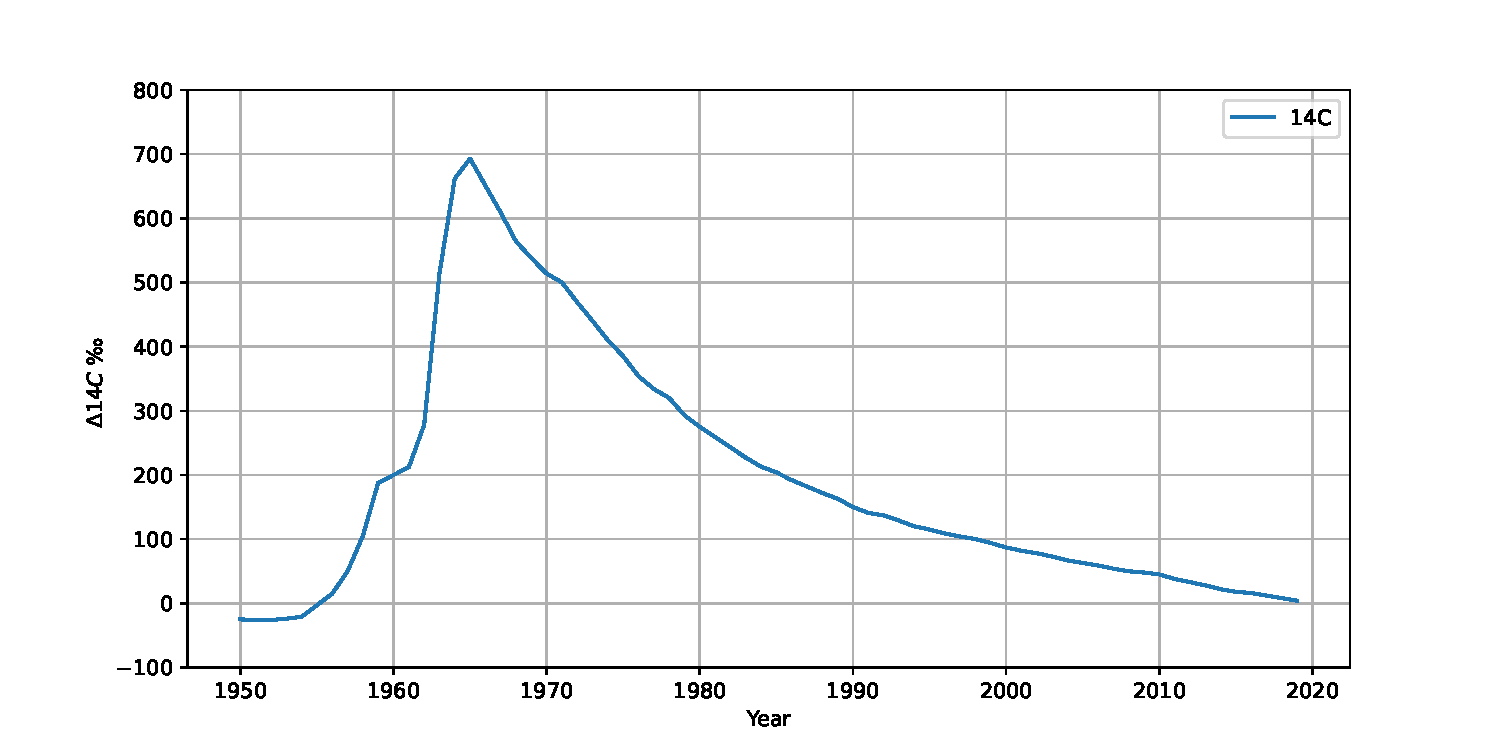
\includegraphics[scale=0.4]{../img/bombcurve.pdf}
    \caption{Concentration of 14C relative pre-industrial time.}
    \label{fig:bomb-curve}
  \end{subfigure}%
  \begin{subfigure}{.5\paperwidth}
    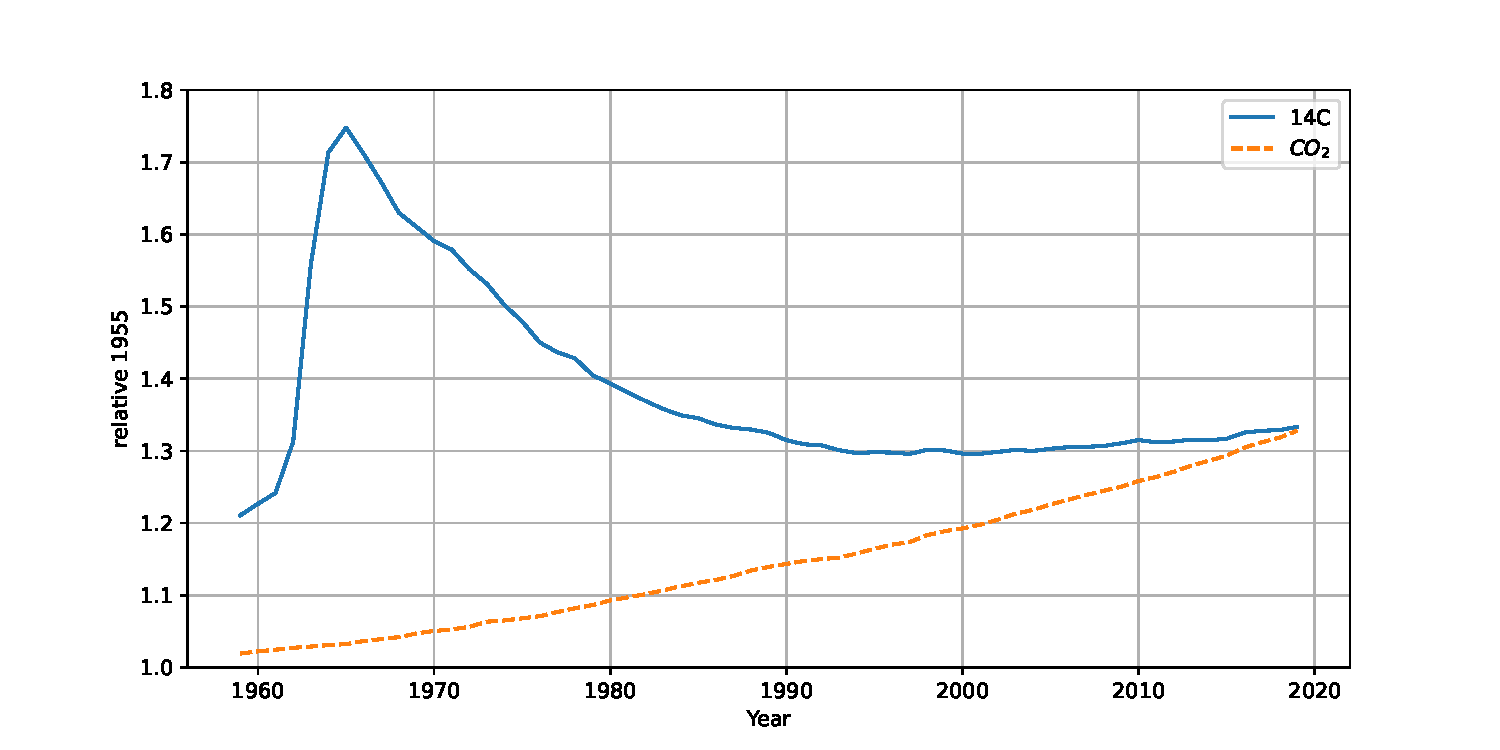
\includegraphics[scale=0.4]{img/relative55.pdf}
    \caption{Amount of 14C and C, relative 1955.}
    \label{fig:relative55}
  \end{subfigure}
  \caption{Carbon-14 in atmosphere}
\end{figure}


In Fig. \ref{fig:bomb-curve} we see the 14C concentrations in the
atmosphere, compared to pre-industrial concentrations (difference
between measured concentration and pre-industrial concentration
divided by pre-industrial concentrations). This series has been
compiled by Quan Hua Chan et.al \cite{Hua:22} and is based on a
atmospheric sampling and tree rings. The concentration is estimated to
have dropped by five percent by 1950 due to the so called Suess effect
(14C free carbon emissions have been added to the atmosphere). As is
clearly seen the 14C concentration rapidly goes up during the
atmospheric testings and then reaches a peek in 1965 (bomb generated
14C initially affected the stratosphere and it took two years for it
to be evenly distributed in the troposphere).

The rapid decline is apparent - carbon dioxide in the atmosphere is
quickly mixing with other reservoirs and the excess 14C quickly goes
away. However, when we interpret these numbers we need to be careful
- what is measured is the concentration of 14C not the total amount of
14C. To estimate the amount of 14C we need to take into account that
the atmosphere now contains more carbon dioxide, compared to the mid
fifties. In Fig. \ref{fig:relative55} we have taken this into account
and show the amount of 14C relative to the amount in 1955. We also
show how the total amount of carbon dioxide has grown since 1955.

The 14C curve in in Fig. \ref{fig:relative55} shows how the bomb
experiments quickly raise the amount of 14C in the atmosphere to
$75\%$ above the 1955 levels. It then quickly decreases until
1994 where it levels off and then slowly increase. Any physical model
that we build should be able to recreate this process. 

\subsection*{the statistical analysis}

Given the information from the bomb curve we can estimate the
unknowns. If we look at Fig. \ref{fig:fit} we see the best fit given a
combined linear and exponential function. The result is the function:

$$
   C14(t) = 0.74 \times e^{-t/17} + 0.0055\times t + 1
$$

The exponential and the linear functions are shown in
Fig. \ref{fig:terms}. We now sea that the exponential decay continues
and how the linear component counter the decay and takes over at
around 1994. This is not exactly what is happening but it gives us the
large picture.

\begin{figure}[ht!]
  \centering
  \hspace*{-3cm}
  \begin{subfigure}{.5\paperwidth}
    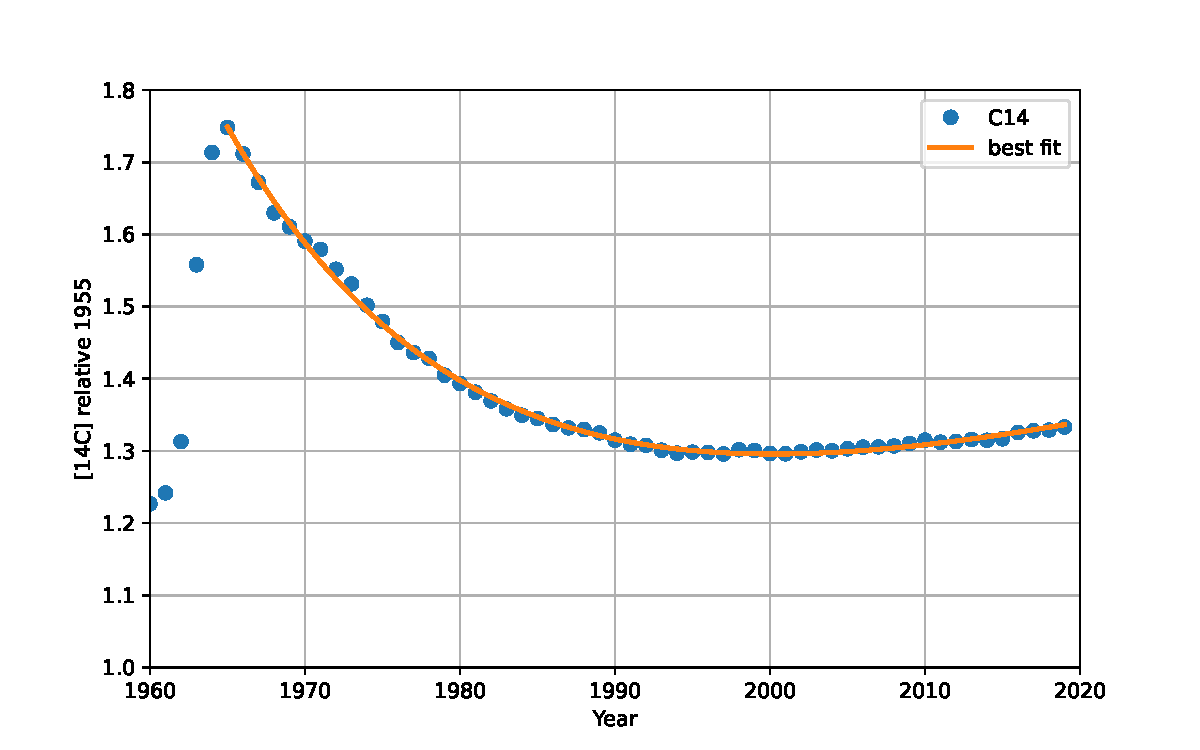
\includegraphics[scale=0.4]{img/fit.pdf}
    \caption{best fit exponential decay}
    \label{fig:fit}
  \end{subfigure}%
  \begin{subfigure}{.5\paperwidth}
    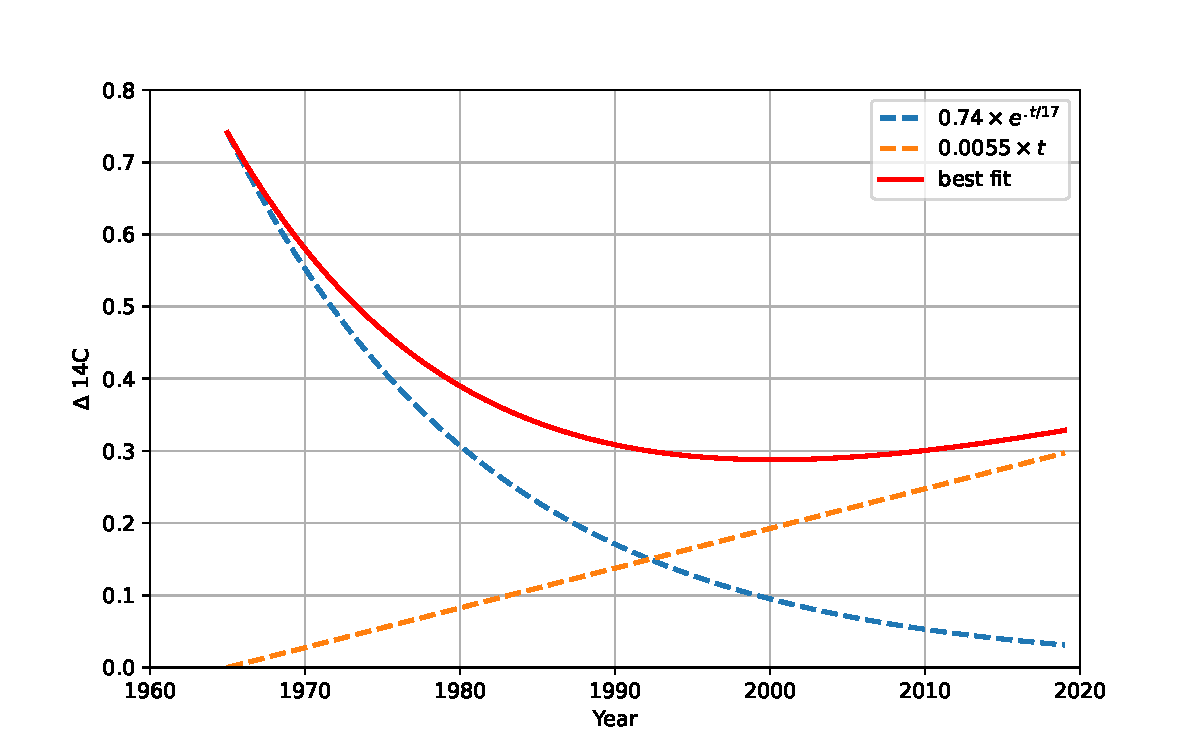
\includegraphics[scale=0.4]{img/terms.pdf}
    \caption{components of the best fit}
    \label{fig:terms}
  \end{subfigure}
  \caption{Exponential and linear components}
\end{figure}

The function that we have is good description of what is actually
happening. If we look at the residual of the measured values and the
best fit description, it is a random function with no trend. It's mean
and median values are both zero, the standard deviation is $0.006$ and
the skewness is $0.7$. If we look at the residual after 1975 the
values are even smaller.

\begin{figure}
   \centering
   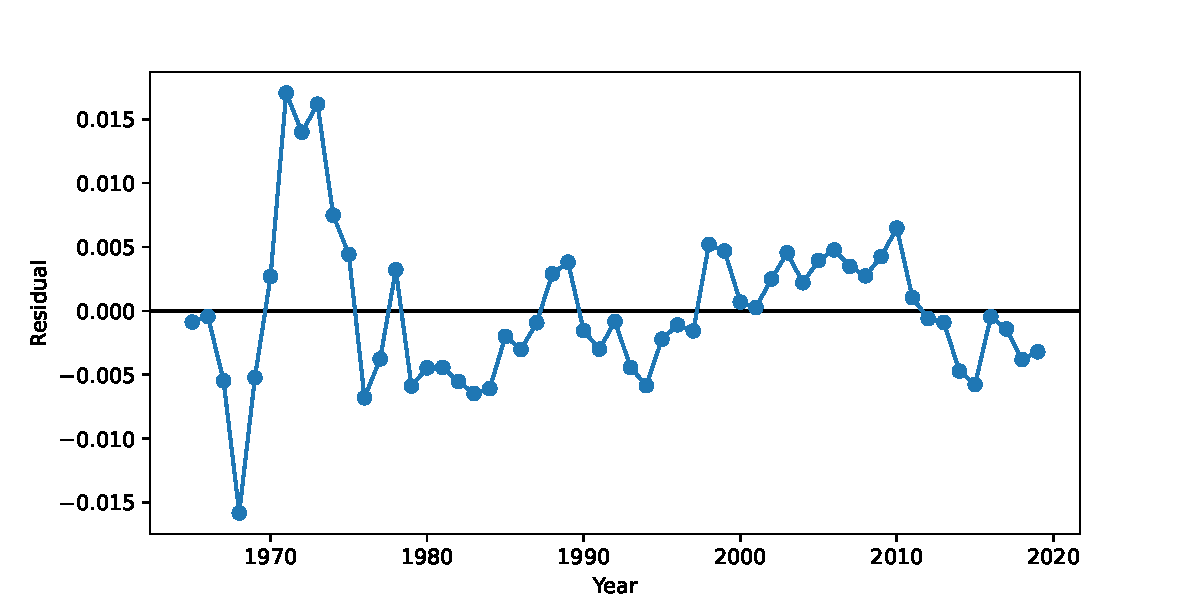
\includegraphics[scale=0.5]{img/residual.pdf}

  \begin{tabular}{ c c c c}
    \textbf{period} & \textbf{std dev} & \textbf{skewness}  & \textbf{linear trend}\\
    \hline\\
    1965-2019 &         0.006 &    0.7 &  0\\
    1975-2019 &         0.004 &    0.1 &  0\\
  \end{tabular}
  \caption{Residual of measured data and best fit equation.}
\end{figure}

The small and random distribution of the residual values indicate that
the statistical model captures the dominating behavior. Our task now
is to create a physical model that shows the same behavior. This will
as we shall see to be a quite tricky task.

\section*{The physical model}

The model that we should create is a two-box model but we not only
have the flows between the models to handle but our emissions that are
adding carbon dioxide to the atmosphere. When studying the bomb curve
this becomes very important since carbon dioxide from fossil fuel is
free from 14C. Emissions of fossil fuel carbon will thus not only
increase the amount of carbon in the atmosphere but also decrease the
concentration of 14C. This is the so called {\em Suess effect} and it
must be taken into account.

We have a small contribution of 14C to the atmosphere each year. One
source i natural galactic radiation that created C14 from
nitrogen. This is a more or less constant process that compensate for
the slow removal and eventual decay of 14C in the carbon
cycle. Another source is 14C created as a side effect in any nuclear
reactor. This contribution, while small, has of course increased as
the number of reactors have increased. In this analysis we will not
take this into account but one should know that they are part of the
picture.

We assume that the flow from the atmosphere to the oceans is
proportional to the amount of carbon in the atmosphere. We have good
data on the amount of carbon emitted from fossil fuel so that should
not be a problem. There should be a flow from the oceans to the
atmosphere and in our simple model where we assume that the oceans
are well mixed this flow should be proportional to the amount of
carbon in the oceans.

We can model this by two reservoirs and differential equation that
determines the flows. If we do it right we should be able to both
recreate the bomb curve but also the increase in the atmosphere.

\subsection*{a simulation}

The simulation will start in 1965 when the bomb curve peeked. From the
Keeling curve \cite{noaa:co2} give us the amount of carbon in the
atmosphere. We have good numbers of the yearly emission \cite{gcb},
and the left is to determine the size of the ocean the rate of flow
between the reservoirs.

The following equations would determine the amount of carbon in the
atmosphere, $A(t)$, and the ocean, $O(t)$. The emissions one year,
$E(t)$ will be in the atmosphere the next year. The rate of flow,
$k_a$ and $k_o$, are of course to be determined and so is the size of
the ocean, expressed as, $x$, multiple of the atmosphere. 

\begin{align*}
  A(0) &= 682 \ \text{GtC} \\
  A(t) &= A(t-a) - k_a \times A(t-1) + (1 - k_o) \times O(t-1) + E(t-1) \\
  \\
  O(0) &= x \times A(0) \ \ \text{\em x is unknown}\\
  O(t) &= k_o \times O(t-1) + (1 - k_a) \times A(t-1)\\
\end{align*}

The rate of the flow from the atmosphere is expressed as an
exponential expression given the residence time $\tau$.  The rate from
the ocean is set to a rate that will make the flows equal in size at
the start of the simulation. The simulation should therefore
determine only $\tau$ and $x$.

\begin{align*}
  k_a &= (1 -  e^{-1/\tau}) \\
  k_o &= \frac{k_a}{x}
\end{align*}


\begin{figure}
  \centering
  \hspace*{-3cm}
  \begin{subfigure}{.5\paperwidth}
    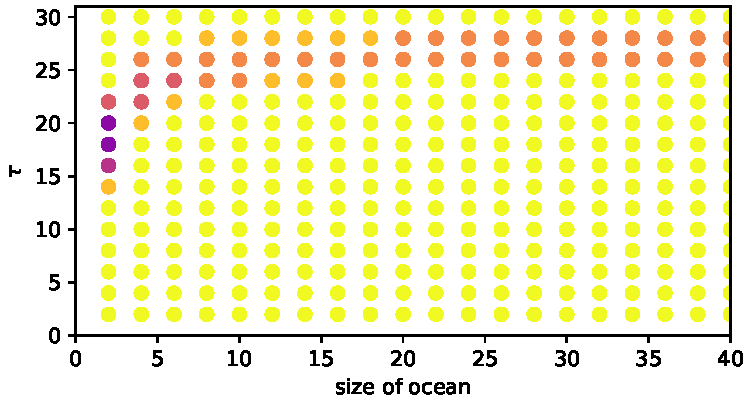
\includegraphics[scale=0.6]{img/keeling-heat.pdf}
    \caption{Amount of carbon.}
    \label{fig:keeling-heat}
  \end{subfigure}%
  \begin{subfigure}{.5\paperwidth}
    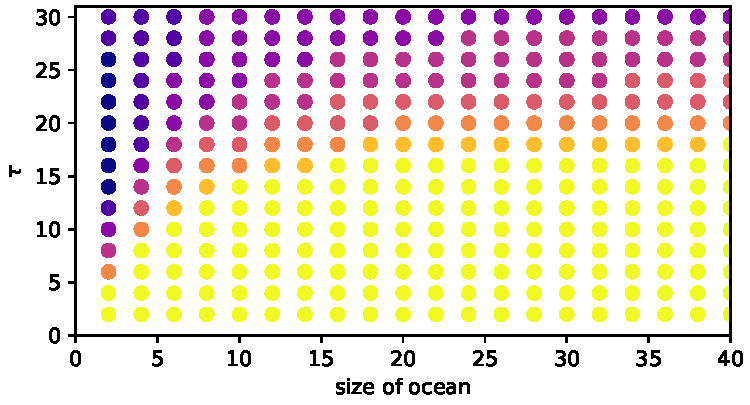
\includegraphics[scale=0.6]{img/bomb-heat.pdf}
    \caption{Concentration of 14C.}
    \label{fig:bomb-heat}
  \end{subfigure}
\end{figure}


\subsection*{a first try}

In out first try we only look at the total amount of carbon in the
atmosphere and try to determine the unknowns. In
Fig. \ref{fig:keeling-heat} we see a heat map of the mean squared
error given the simulation and the measured values of the amount of
carbon in the atmosphere. As seen the simulation favors a comparably
small ocean with a short residence time. As the size of the ocean
increase the residence time increase, favoring approximately 25 years.

If we zoom in we fond that the lowest mean squared error is found when
the size of the ocean is only $0.9$ times the atmosphere and the
residence time is only five years.  The size does of course explain
why the amount of carbon in the atmosphere has grown with roughly half
the amount of emissions during the period. If the ocean is larger the
residence time needs to be much higher but then the correlations is
not as good.

\subsection*{a second try}

In our second try we instead compare the simulated atmospheric 14C
concentrations to the measured values, In Fig. \ref{fig:bomb-heat} we
see that a wider range of acceptable values. The size of the ocean
should still be small but the residence time could be larger. If we
zoom in we will find a simulation where the ocean is $1.7$ times
larger than the atmosphere and the residence time is 18 years.


\subsection*{comparison}

We now have two best estimates of the unknown values. In
Fig. \ref{fig:keeling-fit} we see the two best fit series and how they
compare to the measured amount of carbon in the atmosphere
(keeling). As clearly seen we have a almost perfect fit with the
estimates that we derived from the first simulation. The series
derived from the second equation does overestimate the initial
increase but is in the end an almost perfect match.

If we look at Fig. \ref{fig:bomb-fit} we see how the two series
compare to the measured concentration (bomb) of 14C in the
atmosphere. The extremely short residence time of the first simulation
courses the concentration to initially drop dramatically but since the
size of the ocean is so small it then levels off. The series derived
from the second simulation is an almost perfect fit.

\begin{figure}[t]
  \centering
  \hspace*{-3cm}
  \begin{subfigure}{.5\paperwidth}
    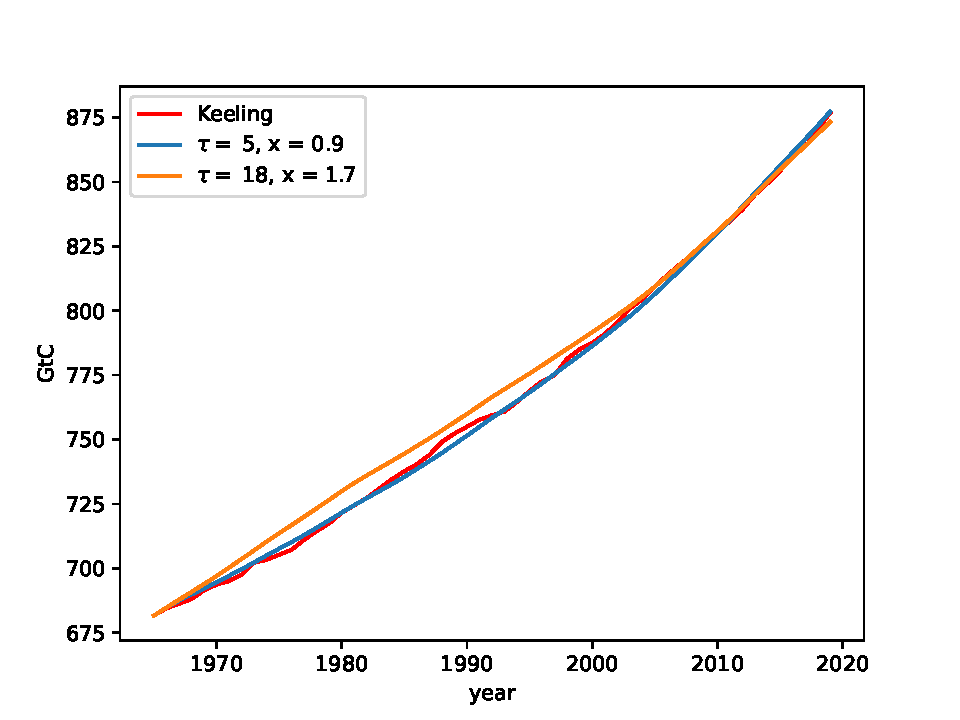
\includegraphics[scale=0.6]{img/keeling-fit.pdf}
    \caption{Amount of carbon  in the atmosphere.}
    \label{fig:keeling-fit}
  \end{subfigure}%
  \begin{subfigure}{.5\paperwidth}
    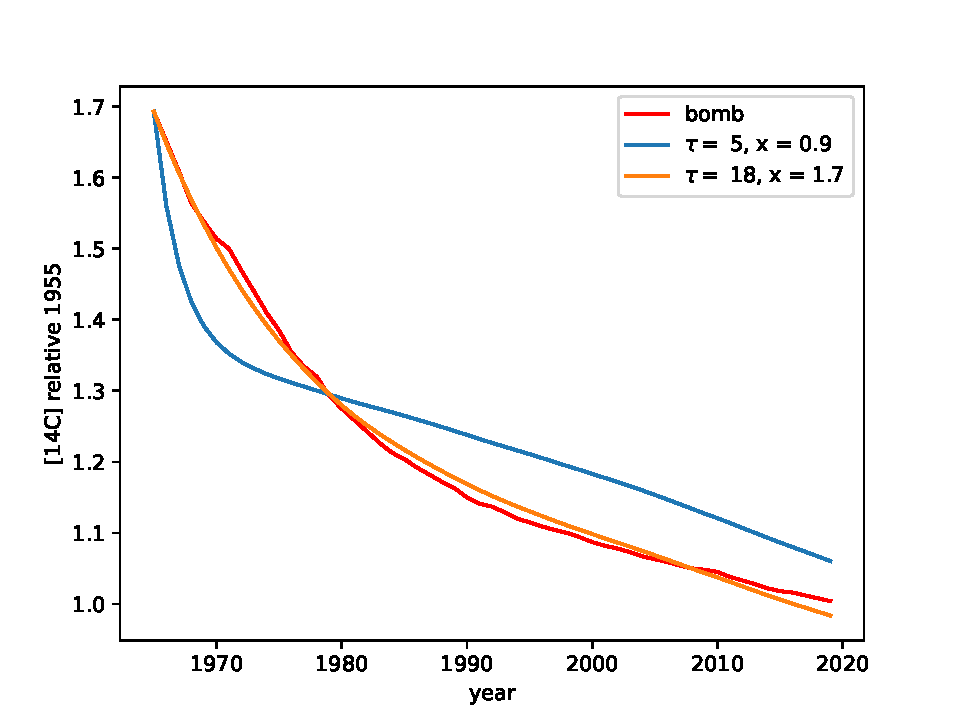
\includegraphics[scale=0.6]{img/bomb-fit.pdf}
    \caption{Concentration of $14C$ in atmosphere.}
    \label{fig:bomb-fit}
  \end{subfigure}
  \caption{The dilemma}
\end{figure}

So we have a simple physical model that can explain both the increase
of carbon dioxide in the atmosphere during the last sixty years as
well as the change in 14C concentrations. The simulation favors a
small ocean reservoir, in size of the same magnitude as the
atmosphere, and a short residence time.

\begin{align*}
  \tau &= 18\\
  x = &= 1.7
\end{align*}

The question now is if this model also can explain the increase that we have seen since 1850.

\subsection*{growth since 1850}

Since we have good estimates on fossil fuel consumption since 1850 we
can run a simulation and see how well it explains current levels of
carbon dioxide in the atmosphere. If we assume that the concentration
in 1850 was 280 ppm equivalent to 596 GtC, we can see the result in
Fig. \ref{fig:century}. As clearly seen the model under estinates our
currentvalues; changing the parameters does improve things but then the
rate of growth is exagerated.


\begin{figure}
   \centering
   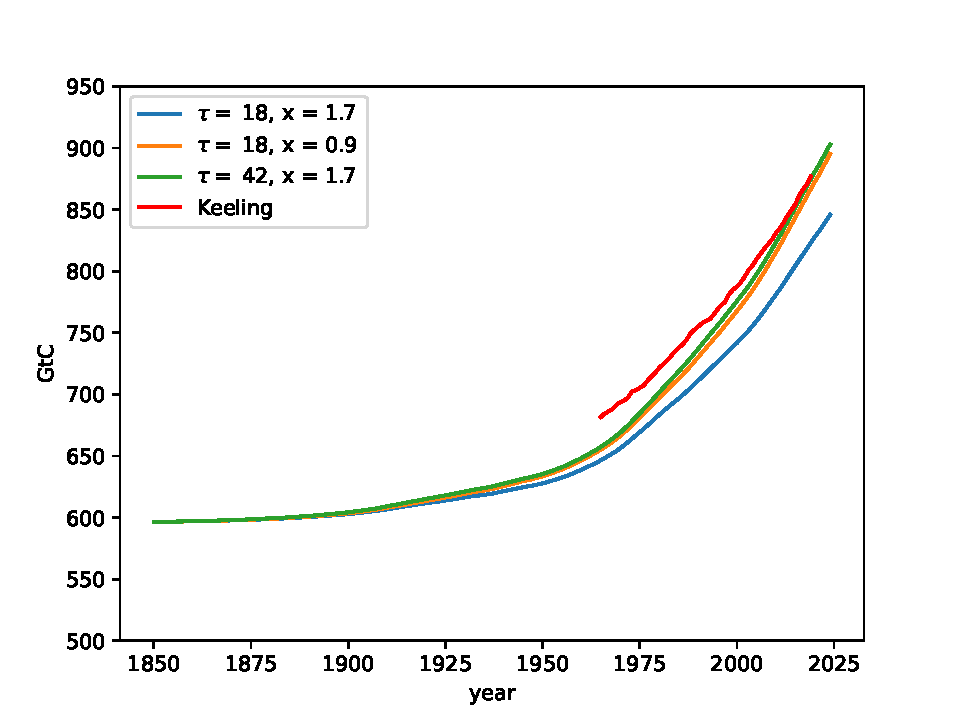
\includegraphics[scale=0.5]{img/century.pdf}
   \label{fig:century}
   \caption{Simulated growth of carbon dioxide in atmosphere since 1850.}
\end{figure}

Given 



\bibliographystyle{plain} % We choose the "plain" reference style
\bibliography{../bib/carbon} % Entries are in the refs.bib file


\end{document}
